\subsubsection{Überblick}
\begin{itemize}
\item Datnepaket-Dienst
\item Dynamische Bündelung freier Slots zu hochbitratigen Datenkanälen, je nach coding Schema 8 bis 21.4 kbit/s
\item asymetrische Übertragung - Slots werden nur belegt, wenn effektiv übertragen wird
\item Gebühren nach Datenmenge und nicht mehr nach Zeit
\item Standartisierung 1998, Einführung 2001/2002
\item Erweiterung der bisherigen Netztopologie
\item geplant ist ein komplementärer Einsatz von GSM/GPRS und UMTS
\item Harmonisierung Internet und Mobilnetz dank IP
\end{itemize}
\subsubsection{GPRS Netzelemente}
\begin{itemize}
\item GSN: GPRS Support Nodes
\begin{itemize}
\item GGSN Gateway GSN - Gateway zu PDNs(Public Data Network)
\item SGSN Serving GSN - unterstützt die MS(location, billing security)
\end{itemize}
\item GR: GPRS Register - eine Ergänzung zum HLR zur Adressverwaltung
\item PCU Packet Control Unit - Übernimmt BSC Funktion im paketorientierten Netzwerk
\end{itemize}

\subsubsection{Architektur Übersicht}
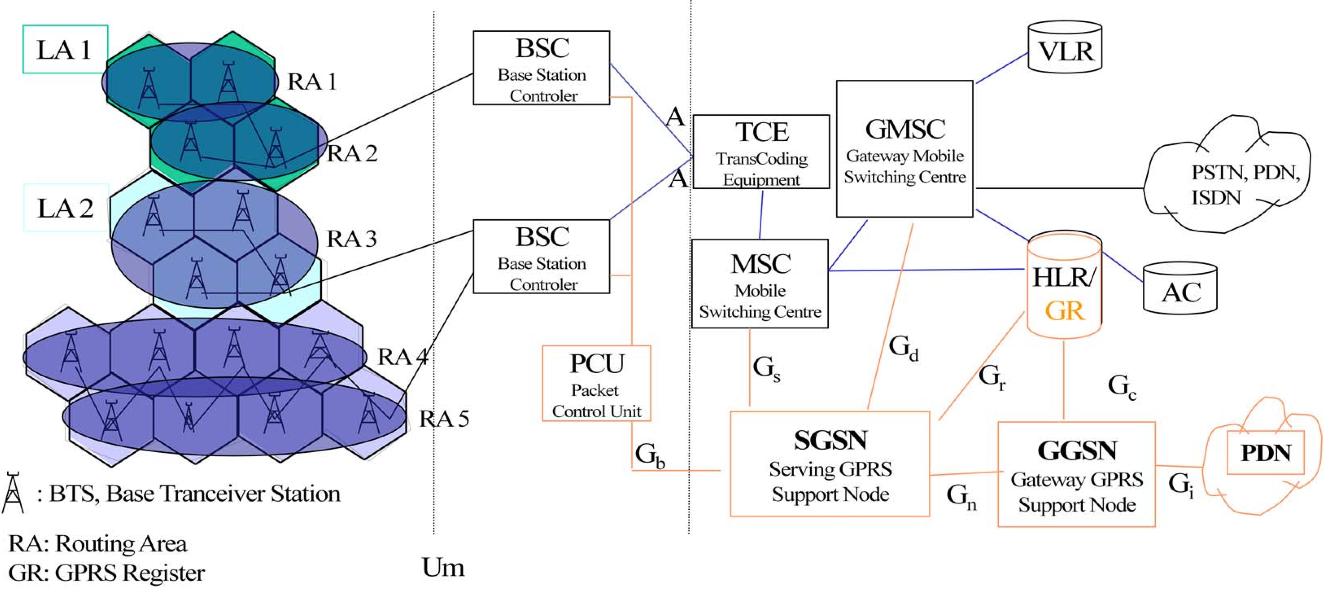
\includegraphics[width = \linewidth]{./Pics/GPRS.png} \\
Diese Grafik zeigt sehr gut, dass das GPRS kein neues Netz ist sondern eine Erweiterung von GSM. Orange eingefärbt sieht man die neuen Element. Man hat nun neben dem Verbindungsorientierten GSM Netz noch ein Paketorierntiertes GPRS Datennetz. Dieses Netz wird ausschliesslich zur Datenübertragung verwendet und kann wegen einer sehr hohen latenzzeit (bis 500ms) auch nicht für VOIP verwendet werden.

\subsubsection{Protocol stack}
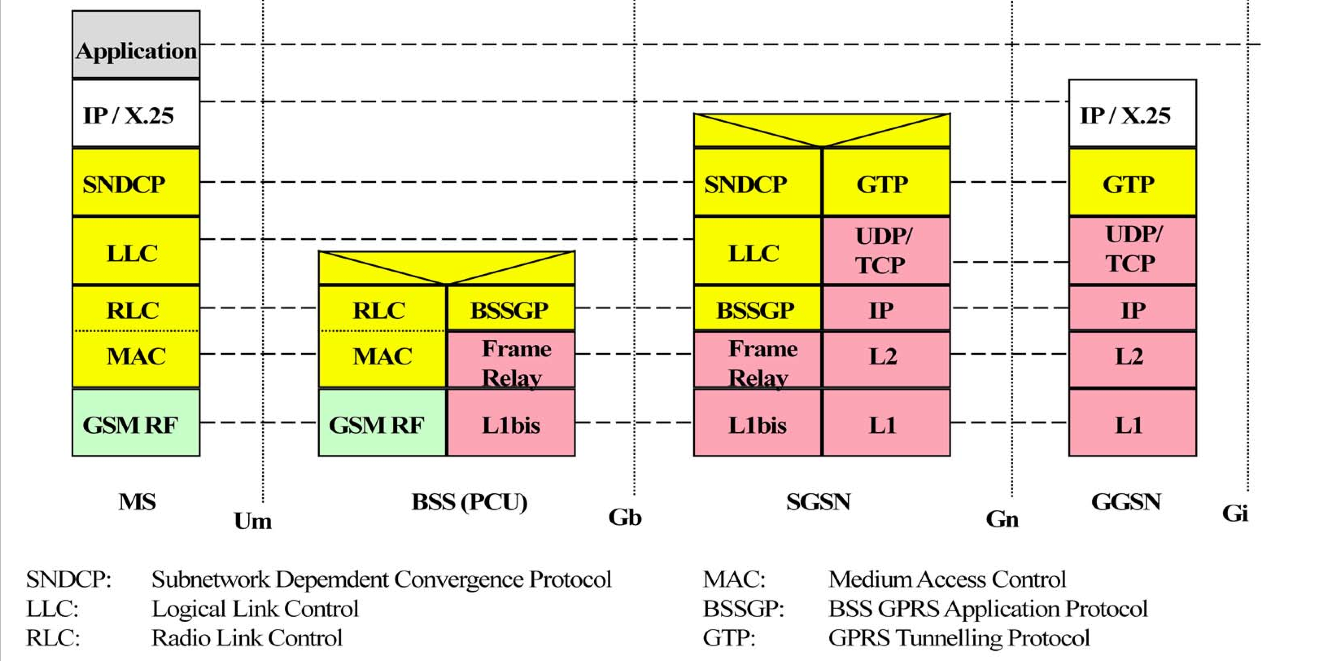
\includegraphics[width = \linewidth]{./Pics/GPRS2.png}

\begin{tabular}{|l|l|l|l|}
\hline
IP & Internet Protocol & X.25 & vorläufer von IP \\
SNDCP & Subnetwork Dependent Convergence Protocol & LLC & Logical Link Control \\
RLC  & Radio Link Control  & MAC & Medium Access Control \\
GSM RF &  Global System for Mobile Communications Radio Frequencies & BSSGP & Base Station System GPRS Protocol \\
GTP & GPRS Tunnelling Protocol & UDP & User Datagram Protocol \\
TCP & Transmission Control Protocol & & \\ 
\hline
\end{tabular}
\subsubsection{GTP}
Das GPRS Tunnelling Protocol baut IP-basierte Verbindungen durch den Backbone auf. Datenpakete werden eingepackt \& unter Benutzung des GTP getunnelt. GTP nutzt unterhalb TCP oder UDP  abhängig von der Nutzeranforderung. Das ganze GPRS Netzwerk basiert auf einem IP Hop, was das Routing im Backbone bei Mobilität vereinfacht.
